%Chapter 4: Kinematic Source Inversions

\chapter{Kinematic Source Inversions}

In Chapter 3 we discussed a framework for static slip inversions. Elaborating on the work of \citet{Crowell2012} we demonstrated it is possible to construct static models for large earthquakes objectively with minimal interaction from a human operator. Static dislocation models are limited in the sense that they provide only the total slip on the assumed rupture surface and provide no information on the time evolution of rupture. They are just a before and after snapshot of the event.  They do not illuminate important kinematic parameters of the rupture process; how fast was the rupture? What is the shape of the source time function, both at individual sub-faults and for the earthquake as a whole? Answers to questions like these have important implications not only for hazards applications but to furthering our understanding of the physics that governs the rupture process.

\section{Background}

\label{sec_backgr}

As instrumental seismology matured in the mid 20th century and observatory grade seismological stations and strong motion sensors proliferated it became possible to consider kinematic models of the earthquake source process. Perhaps the first successful macroscopic model, containing simple parameters, was the Haskell fault model \citep{haskell1964,haskell1969} which consisted of a rectangular fault with constant, unidirectional rupture velocity (a boxcar source time function). It successfully explained phenomena such as directivity and made predictions about the shape of source spectra. This propagating dislocation model was successfully used to model data observed at only 80m from the fault trace of the 1966 Parkfiled earthquake \citep{aki1968}.

As systematic studies of source properties evolved it became apparent that large earthquakes had more complexity than a simple propagating line source with a prescribed rise time and rupture velocity and homogenous slip. Indeed it was clear that some events could only be modeled by relaxing these constraints. \citet{kanamori1978} demonstrated that the far field body waves of the 1976 $M_w$7.6 Guatemala earthquake were best explained by superposition of ten sources, while \citet{trifunac1974} employed strong motion records of the 1971 $M_w$ 6.6 San Fernando earthquake to solve the first heterogeneous slip inversion proper.

Following the 1979 $M_w$6.4 Imperial Valley earthquake, which was well recorded by numerous strong motion stations, an efficient way to parametrize the temporal and spatial variations of the source and invert for them was defined. \citet{olson1982} and \citet{hartzell1983} introduced what is now known as the \textit{multi-time window} method, whereby slip on a sub-fault is allowed to occur over contiguous time windows. In this way heterogeneities of the spatial and temporal behavior of the fault can be modeled.

Formally, an inversion problem for the time dependent slip of an earthquake can be set-up by discretizing an assumed fault surface into a grid of $N$ sub-faults. Then, the response at a given station can be computed from
\begin{equation}
\label{eq:slip}
u(t)=\sum_{j=1}^ND_j[\cos(\lambda_j)G_j^{ss}(v_j,t)+\sin(\lambda_j)G_j^{ds}(v_j,t)]\dot{S}_j(t)\;,
\end{equation}
where $u(t)$ is the displacement seismogram at a given station and $D_j$ the dislocation amplitude at the $j$-th sub-fault. The dislocation is decomposed into its strike-slip ($ss$) and dip-slip ($ds$) contributions by taking the cosine and sine, respectively, of the rake angle $\lambda$. $G^{ss}(v,t)$ and $G^{ds}(v,t)$ are the dip-slip and strike-slip Green functions which represent the response of a point, impulsive source. $\dot{S}(t)$ is the source time function which regulates the temporal dependence of moment release at a subfault. The Green functions depend on the rupture velocity, $v$ insofar as they need to be delayed by the time required for the rupture to propagate from the hypocenter to each subfault. Evidently, if the timing of slip is considered an unknown quantity, then the general expression in Equation \ref{eq:slip} is non-linear. Furthermore the source time function itself must be parametrized, the choice of such parametrization will also have an effect on the linearity of the problem.

Indeed, the main difference in the approaches to the kinematic slip inversion is that of the assumption of linearity. To treat Equation \ref{eq:slip} as linear one can assume a rupture speed  and allow slip at each sub-fault to happen in one or many subsequent time windows following the main arrival of the rupture front \citep{olson1982,hartzell1983}. The source time function can be parametrized in a number of ways, usually overlapping triangles or boxcars, but is in general treated as being decomposed into basis functions \citep{ide1996}. In this way the inversion is linear an can be solved with any of the usual algorithms. Typically a nonnegative least squares (NNLS) solver is employed \citep{lawson1974} to prevent the direction of slip from reversing. In this inversion approach it is important to have sufficient time windows, or basis functions, to allow for some complexity in the time evolution of slip. If the parametrization is overly simple then unexpected errors can occur in the final result \citep{hartzell1993}.

If the timing of slip is treated as an unknown quantity the non-linear inverse problem can be solved provided one assumes a parametrization of the source time function $\dot{S}$. Thus, in this approach the rupture is linear with regards to the amount of slip but non-linear with regards to its timing. Of benefit in this inversion scheme is that source time functions whose shape is based on rupture dynamics can be used. Examples of this can be found in \citet{beroza1988} who use a source time function derived from dynamic crack propagation and \citet{ji2003} who use a source time function that simulates a starting and stopping phase. Non-negativity can still be enforced in the non-linear case by employing an error function that grows asymptotically as slip approaches 0 \citep{yoshida1990}. These non-linear approaches however, use only one time window per subfault and cannot model complex source time histories. The importance of this remains unclear, there is uncertainty as to the robustness of complex source time functions obtained with the linear method. \citet{ide2007} compared several linear and nonlinear inversions for the $M_w7.6$ Chi-Chi, Taiwan earthquake and found that while the gross features of slip are consistent amongst studies there can be significant variations in the timing of slip. \citet{ide2007} also found that models that include geodetic data show improved consistency.

There is also a class of slip inversions that analyzes the data in the frequency domain. This has been a less popular but well studied approach. The first solutions in the frequency domain were reported by \citet{olson1988} and \citet{cotton1995}. Later \citet{ji2002} proposed a more innovative approach by using wavelet analysis to quantify the contributions of finite frequency signals to the slip inversion. These methods, as well as the time domain ones, independently of the data type used, far- or near-field, rely on low pass filtered time series, they depend on the long period component of the seismic record for the inversion. This choice of data type can have an effect on the final model, furthermore, whether the time series are studied as velocity or displacement waveforms can also affect the inversion result \citep{ide2007}. velocity waveforms tend to display higher levels of high frequency waves, while displacement waveforms are dominated by long period energy. Due to this large suite of options available to the seismologist who wishes to study the time dependent behavior of earthquake rupture, there is still a lot of heterogeneity in the results reported by independent research groups for any given earthquake. Nonetheless, kinematic inversion has become a routine analysis and important tool for the study of medium to large events.

For rapid response the USGS routinely produces automated slip inversions for large events using the wavelet method of \citet{ji2002} and relying on far field body and surface waves. These models are computed several hours after the event and are usually the first source of kinematic information about large events. Inversions with regional data are only performed in post processing. They typically rely on baseline corrected or high-pass filtered strong motion data. Recently, for example, \citet{suzuki2011} inverted strong motion data from the $M_w$9 Tohoku-oki event using the multi-time window method. In that study the acceleration waveforms were integrated once to velocity and band-pass filtered between 100s and 8s. The results show a smooth slip distribution with large slip near the trench. However, approaches such as this one for regional inversions are limited. Consider figure \ref{fig_myg011} where we have applied a bandpass filter between 100s and 8s to the east component of station MYG011. This is the same procedure as that in \citet{suzuki2011} (station MYG011 was used in that inversion). The figure shows the filtered accelerogram integrated to velocity and then displacement. Notice that the filtering operation has eliminated the static field and the integrated displacement waveform compares very poorly to the collocated GPS station. it is not mentioned in that study how the smoothing parameters were selected, but, it is difficult to consider a model which does not constrain the static field a robust one. it is still informative, but, for certain applications, such as tsunami modeling not of much use.

An alternative approach is to directly invert high-rate GPS data. Given the problems with signal aliasing discussed in Chapter 2 and the elevated noise levels, especially in the vertical channel it is only advisable to invert the longer period portion of the GPS recording. For example \citet{yue2011} low-pass filtered GPS recordings of the Tohoku-oki event at 80mHz. This approach yields very smooth models which tend to be very similar to simple static models derived just from coseismic offsets. It is easy to understand why; at such long periods the largest signal in the time series is the coseismic ramp. Higher frequency waves are obscured and there is only limited information about the time dependent rupture process. Differentiating the GPS time series to velocity is not advisable because of the slow sampling rates and high noise.

Thus the Kalman filter solution which provides both reliable velocity and displacement waveforms that contain information across a broad frequency range seem well suited for kinematic inversion at regional distances. We will demonstrate in the following pages that this is indeed the case.

\begin{figure}[!ht] 
  \centering
  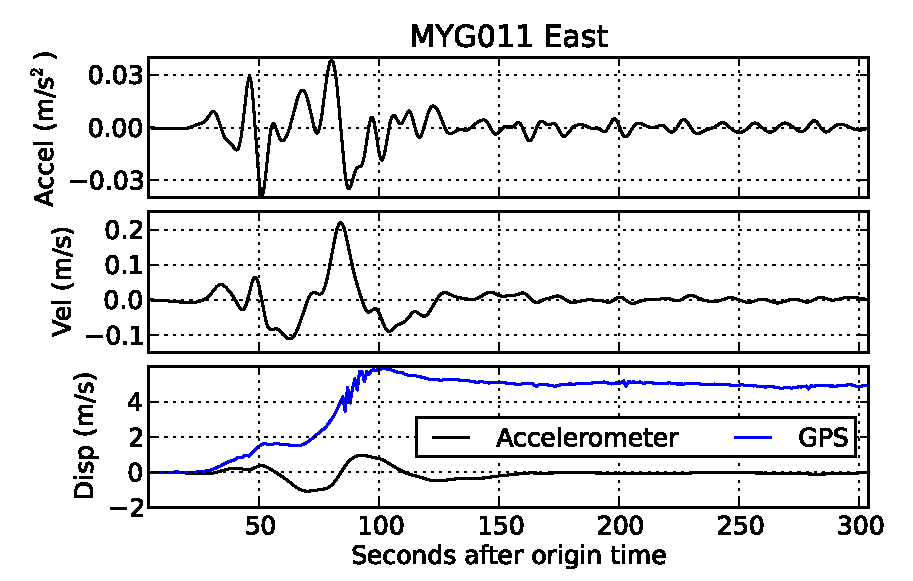
\includegraphics[width=0.9\linewidth]{./figures/ch4/myg011_vel.pdf}
    \caption[Bandpass filtered waveforms for MYG011]{Results of bandpass filtering the accelerometer recording at station MYG011 and integrating it to velocity and displacement}
  \label{fig_myg011}
\end{figure}


\section{The Inverse Problem}

Throughout this chapter we will employ for our analysis the multi-time window method. Following \cite{ide1996} we can consider the decomposition of the source time function at the $j$-th subfault into $K$ basis functions
\begin{equation}
D_j\dot{S}_j(t)=\sum_{k=1}^Kb_k\phi_k(t)\;,
\end{equation}
where $b_k$ is the expansion coefficient of the $k$-th basis function $\phi_k(t)$. In the multi-time window approach we consider overlapping basis functions with a simple geometry. Commonly used are b-splines with equally spaced knots which yield a simple isosceles triangle shape \citep{ide1996,wu2001}. 
Thus, one assumes a maximum rupture velocity $v^{max}$ and then allows slip on subsequent \textit{windows}  which are offset at regular time intervals, typically 50\% of the of the rise time of the triangle basis function. In this way we've effectively linearized the problem by assuming known rupture times, while still allowing flexibility in the timing of slip by permitting dislocations at later times after the maximum rupture velocity time. The inverse problem will now be a solution for the expansion coefficients $b_k$ which represent the amplitude of each triangle source time function at each sub-fault for strike- and dip-slip motions yielding a total of $2KN$ model parameters.


Green's functions must be computed numerically. If one assumes Earth structure is a 1D layer-cake model then at regional distances (hundreds to a couple thousand kilometers) GFs can be obtained by the frequency-wavenumber (fk) integration method \citep{saikia1994}. Importantly, the fk method is capable of computing the ultra-long period band of the seismogram down to the 0 frequency static offset \citep{zhu2002}. It can be employed to model strong motion displacement data from the seismogeodetic solution. Other approaches involve normal mode summation \citep{yue2011}. Ideally it would be desirable to use three dimensional GFs for the inverse problem solution. This is a computationally intensive operation, sometimes prohibitively so. However, it is becoming prevalent to use fully 3D Earth models for forward computation of wave propagation \citep{bielak2010,tromp2010}. As our knowledge of Earth structure progresses it will become important to consider more complex velocity models. However, 3D velocity models only exists for a very small fraction of the Earth and while \citet{graves2001} and \citet{wald2001} demonstrated that 3D structure enhances model resolution, they also showed that this improvement is only possible with accurate 3D models. In fact they demonstrated that a well calibrated 1D model is preferable over an imprecise 3D Earth model.

Thus, with Green functions in hand we can set up the traditional linear inverse problem, as in Chapter 3:
\begin{equation}
\label{eq:inv}
\mathbf{GM}=\mathbf{d}\;,
\end{equation}
where the data column-vector $\mathbf{d}$ is the concatenation of observed seismograms at all stations, the Green functions $\mathbf{G}$ are the motions at every station from every subfault for a triangle source time function of given rise-time and the model parameters $\mathbf{m}$ are the amplitude of the allowed source time functions at each sub-fault. As in the static case $\mathbf{G}$ is not full rank. Even though this is an over-determined problem the data are not always independent and parts of the model often cannot be resolved by the data. This rank deficiency produces a large condition number which effectively yields extremely irregular models with sharp, unphysical variations between neighboring subfaults and overlapping time windows. Regularization must be employed; one popular form of regularization in slip inversions is to fix the total amount of seismic moment at a value suggested from other sources \citep{ji2002b}. However for our case we prefer moment be determined by the data themselves. Rather, we employ a spatial and a temporal regularization to increase the effective rank of the problem. For the spatial regularization we use the Laplacian finite difference operator as in the static case of Chapter 3. We request that the sum of the slip of all windows at a given sub-fault be smooth in this sense. This penalty function is applied only to the total slip, not to the individual time windows. For a temporal regularization we apply a simple first derivative penalty function to each subfault's windows, such that sharp variations between the amplitudes of contiguous time-windows are possible but discouraged. 

\subsection{Spatial Regularization}

For slip inversions we have relied on the finite difference Laplacian operator for spatial regularization. For static inversions in Chapter 3 we used the traditional 5 point stencil approximation to the Laplacian. At a given sub-fault (position $i,j$) the 4 neighboring sub-faults are used to compute the finite difference Laplacian of a given component of  slip $m_{ij}$ as
\begin{equation}
\label{eq_laplace1}
\nabla^2m_{i,j}=\frac{-4m_{i,j}+m_{i+1,j}+m_{i-1,j}+m_{i,j+1}+m_{i,j-1}}{h}\;,
\end{equation}
where $h$ is the distance between the center's of the sub-faults. If it is constant then the term can be treated as unity. This formulation is easily derived by applying the second order accurate expressions for the second derivative in the along strike and along dip directions.  The situation is illustrated schematically in Figure \ref{fig_stencil} and the computational molecule for a slip patch within the model is in Figure \ref{fig_molecules}a  A survey of the literature will reveal that seldom do authors indicate what course of action to take at the edges of the model. At the boundaries of the fault one can simply drop one term of Equation \ref{eq_laplace1} (or two if you are at a corner). For example at the top edge of the fault model  (Figure \ref{fig_stencil}, position $i,1$) we would write
\begin{equation}
\label{eq_laplace2}
\nabla^2m_{i,1}=\-4m_{i,1}+m_{i+1,1}+m_{i-1,1}+m_{i,2}+0\;,
\end{equation}
where we have set $m_{i,0}=0$. This simplifies the computational molecule from 5 elements to 4 (Figure \ref{fig_molecules}b). Indeed, this is equivalent to assuming that there exists a ghost cell $m_{i,0}$ beyond the edge of the fault model that has no slip. This is a reasonable assumption for a buried fault where slip must taper off towards the edges. This regularization, while not precluding slip at the fault boundary, will put a large penalty on it. Large slip at the edge will mean a large derivative and will be discouraged in the inversion

\begin{figure}[!ht] 
  \centering
  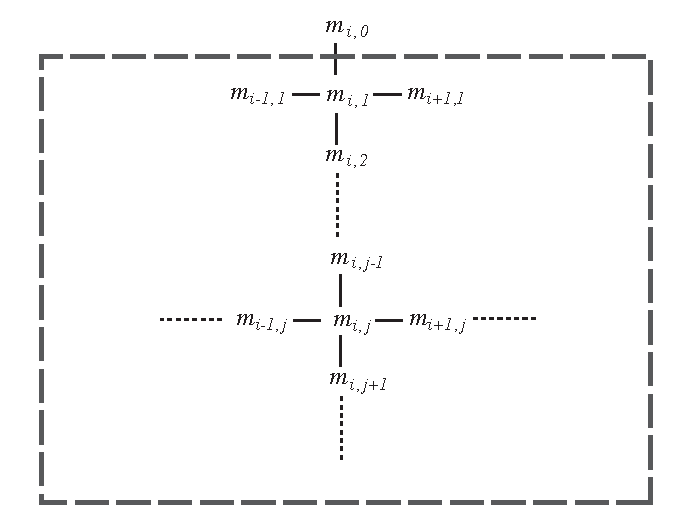
\includegraphics[width=0.75\linewidth]{./figures/ch4/laplace_stencil.pdf}
    \caption[Stencil for finite difference laplacian]{Stencil for finite difference laplacian}
  \label{fig_stencil}
\end{figure}

\begin{figure}[!ht] 
  \centering
  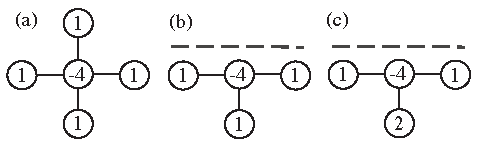
\includegraphics[width=0.75\linewidth]{./figures/ch4/molecules.pdf}
    \caption[Computational molecules]{Computational molecules for the finite difference laplacian. (a) is somewhere within the fault model. (b) is for a zero-slip condition at the top edge and (c) is a free boundary condition at the top edge.}
  \label{fig_molecules}
\end{figure}

This is problematic for a subduction zone megathrust that extends all the way to the trench. This zero-slip boundary condition is unreasonable since large slip can and should be allowed to happen at the trench. In Chapter 3 we used this boundary condition for the static slip inversion. The result is a model that does not have large amounts of motion at the trench. In order to penalize slip at the top edge of the model less harshly the stencil must be modified. We can instead require that the derivative of slip normal to the fault edge (in the dip direction, index $j$) be zero. If we approximate the first derivative by a second order accurate central difference then at the top edge we have the condition
\begin{equation}
\frac{dm_{i,1}}{dy}=m_{i,0}-m_{i,2}=0\;,
\end{equation}
where once again we assume the spacing between sub fault centers is unity. This free boundary condition means that $m_{i,0}=m_{i,2}$ and yields the expression for the Laplacian at the top edge
\begin{equation}
\nabla^2m_{i,1}=\-4m_{i,1}+m_{i+1,1}+m_{i-1,1}+2m_{i,2}\;.
\end{equation}
Once again we have a 4 point stencil but the computational molecule (Figure \ref{fig_molecules}c) value for the along-dip element has changed from 1 to 2. It is a subtle modification but an important one if slip is to be allowed at the trench. Further on we will demonstrate the effect of this small change to the regularization matrix.


\subsection{Regularization and Bayesian Modeling}

The spatial Laplacian regularization matrix $\mathbf{L}_s$ and the temporal first derivative regularization one $\mathbf{L}_t$ are incorpoated into the problem as
\begin{equation}
\left(\begin{matrix}
\mathbf{G}\\
\lambda_s\mathbf{L}_s\\ 
\lambda_t\mathbf{L}_t
\end{matrix}\right)
\mathbf{m}=
\left(\begin{matrix}
\mathbf{d}\\
\mathbf{0}\\ 
\mathbf{0}
\end{matrix}\right)\;.
\end{equation}
This has the well known canonical solution \citep{menke2012}
\begin{equation}
\label{eq:solution}
\mathbf{m}^0=
(\mathbf{G}^\top\mathbf{G}+\lambda_s^2\mathbf{L}_s^\top\mathbf{L}_s+\lambda_t^2\mathbf{L}_t^\top\mathbf{L}_t)^{-1}
\mathbf{G}^\top\mathbf{d}\;.
\end{equation}
A known complication in this formulation is to objectively decide the values of the smoothing parameters $\lambda_s$ and $\lambda_t$. In Chapter 3, where we have only a spatial regularization, we employed the L-curve curvature criterion \citep{hansen2007}. However such a heuristic criterion is somewhat tricky and quite cumbersome to apply in a two dimensional parameter space. Furthermore it is somewhat unsatisfactory in that it is not grounded in a strictly objective statement about source properties. Often when perusing the literature on slip inversions it is common to find statements that indicate that for a particular study the author used his or her judgment and intuition on the physics of an earthquake to decide on a regularization parameter. This is altogether unsatisfactory, for the slip inversion there exists a probabilistic formalism that can provide objective criteria for selection of the smoothing parameters.

Following \citet{ide1996} we can write the posterior likelihood function, this is a statement about the likelihood of the inversion result, as
\begin{equation}
p(\mathbf{d}|\mathbf{m};\sigma^2)=(2\pi\sigma^2)^{-Q/2}\exp\left[-\frac{1}{2\sigma^2}\|\mathbf{d}-\mathbf{Gm}\|^2\right]\;,
\end{equation}
where $Q$ is the number of data and $\sigma^2$ is the data variance. Without any prior information maximization of this likelihood function will lead to the traditional normal equations \citep{menke2012}. If however, we consider the regularization matrices as a form of prior information we can write the following probability density functions:
\begin{eqnarray}
p(\mathbf{m}|\sigma_s^2)=(2\pi\sigma_s^2)^{-P_s/2}\|\Lambda_s\|^{1/2}\exp\left[-\frac{1}{2\sigma_s^2}\|\mathbf{L}_s\mathbf{m}\|^2\right]\;,\\
p(\mathbf{m}|\sigma_t^2)=(2\pi\sigma_t^2)^{-P_t/2}\|\Lambda_t\|^{1/2}\exp\left[-\frac{1}{2\sigma_t^2}\|\mathbf{L}_t\mathbf{m}\|^2\right]\;,
\end{eqnarray}
where $\sigma^2_s$ and $\sigma^2_t$ are hyper-parameters that represent the smoothing variance. $P_s$ and $P_t$ are the ranks of the two smoothing matrices and $\|\Lambda_s\|$ and $\|\Lambda_t\|$ are the absolute values of the product of the non-zero eigen-values of the smoothing matrices. \citet{ide1996} combined these two pdfs by simple multiplication. However \citet{fukahata2003} subsequently showed that this produces a prior pdf whose integral is not unity and thus is improper. After introducing the correct normalization, the prior pdf that combines both smoothing constraints can be expressed as
\begin{equation}
p(\mathbf{m}|\sigma_s^2,\sigma^2_t)=(2\pi)^{-M/2}\left\|\frac{1}{\sigma_s^2}\mathbf{L}_s+\frac{1}{\sigma_t^2}\mathbf{L}_t \right\|^{1/2}\exp\left[-\frac{1}{2\sigma_s^2}\|\mathbf{L}_s\mathbf{m}\|^2\right]\exp\left[-\frac{1}{2\sigma_t^2}\|\mathbf{L}_t\mathbf{m}\|^2\right]\;,
\end{equation}
where $M$ is the total number of model parameters. We can then use Bayes' theorem to define the posterior pdf of the model as
\begin{equation}
p(\mathbf{m};\sigma_s^2,\sigma_t^2,\sigma^2|\mathbf{d})=Cp(\mathbf{d}|\mathbf{m};\sigma^2)p(\mathbf{m}|\sigma_s^2,\sigma^2_t)\;,
\end{equation}
where $C$ is  a factor introduced to ensure the integral of the pdf is unity. It is, however, independent of the model parameters and hyper parameters and thus not necessary to compute. From this definition of the posterior pdf, \citet{jackson1985} showed that the optimal model $\mathbf{m}^0$ obtained from maximizing the posterior pdf is exactly the damped least squares solution of Equation \ref{eq:solution} where the ratio of the hyperparameters are actually the regularization parameters such that $\lambda_s=\sigma^2/\sigma^2_s$ and $\lambda_t=\sigma^2/\sigma^2_t$. The added benefit of taking the Bayesian approach to deriving the inverse solution is that we can use the posterior pdf to select the optimal regularization parameters.
	
\citet{akaike1980} proposed an information theory and entropy maximization based criterion, now known as the Akaike information criterion (ABIC) for selecting the adequate hyper-parameters. The parameter is obtained from the marginal likelihood as
\begin{equation}
\label{eq:abic}
\mathrm{ABIC}=-2\ln\left[\int p(\mathbf{m};\sigma_s^2,\sigma_t^2,\sigma^2|\mathbf{d})d\mathbf{m}\right]\;,
\end{equation}
thus the optimal model is the one which minimizes information loss and thus has the \textit{smallest} value of ABIC. \citet{fukahata2004} showed that the ABIC can then be expressed as
\begin{equation}
\label{eq:abic_total}
\mathrm{ABIC}(\lambda_s^2,\lambda^2_t)=Q\ln s(\mathbf{m^0})-\ln\|\lambda^2_s\mathbf{L}_s+\lambda_t^2\mathbf{L}_t\|+\ln\|\mathbf{G}^\top\mathbf{G}+\lambda_s^2\mathbf{L}_s+\lambda_t^2\mathbf{L}_t\|\,,
\end{equation}
where $s(\mathbf{m})$ is the residual
\begin{equation}
s(\mathbf{m})=\|\mathbf{d}-\mathbf{Gm}\|^2+\lambda_s^2\|\mathbf{L}_s\mathbf{m}\|+\lambda_t^2\|\mathbf{L}_t\mathbf{m}\|
\end{equation}
and the optimal model $\mathbf{m}^0$ is obtained from the damped solution in Equation \ref{eq:solution}. To use the ABIC to determine smoothing parameters you invert at several values of both smoothing parameters and compute the ABIC value for this regularization pair. Then you select as your final model the one with the smallest value of ABIC. If the smoothing is too strong then the second and third terms in Equation \ref{eq:abic_total} almost cancel each other, but the residual $s(\mathbf{m})$ is large and so is the ABIC. If the smoothing is weak then the residual is small but second term in Eqaution \ref{eq:abic_total} is large and so is the ABIC. The minimum value of ABIC is somewhere between these two extremes and in a sense represents the tradeoff between he residual $s(\mathbf{m})$ and the condition number of the regularized matrix \citep{ide2007}. This approach is a combination of traditional inversion with Bayesian modeling and has been employed by several researchers for kinematic inversions. It has been used, for example, to study the $M_w$ 6.0 Kobe earthquake \citep{sekiguchi2000} the $M_w$7.6 Chi-Chi earthquake \citep{wu2001} and the $M_w$9.0 Tohoku-oki event \citep{yoshida2011}.
A benefit of this Bayesian framework is that if the covariance matrix of the data, $\mathbf{C_d}$ is known then we can compute the covariance of the model parameters as \citep{yabuki1992,ide2007}
\begin{equation}
\mathbf{C}_m=\sigma^2(\mathbf{G}^\top\mathbf{C}_d\mathbf{G}+\lambda_s^2\mathbf{L}_s^\top\mathbf{L}_s+\mathbf{L}_t^\top\mathbf{L}_t)^{-1}\;,
\end{equation}
where
\begin{equation}
\sigma^2=\frac{s(\mathbf{m}^0)}{Q}\;.
\end{equation}
This allows us to make statistical statements about the reliability of a given solution, something that is tricky for traditional high order Tikhonov regularized inverse solutions \citep{aster2013}.


\section{An example with seismogeodetic data, the $M_w9$ Tohoku-oki earthquake}

As discussed in Section \ref{sec_backgr}, for inversion with regional data there are limitations to using just strong motion or high-rate GPS data. We will now demonstrate the performance of the seismogeodetic data for a kinematic inversion of the Tohoku-oki event and argue that it produces a more robust solution than with either data set alone. We select 20 stations from the Kalman filtered dataset described in Chapter 2 and invert the three component displacements and velocities for a total of 120 waveforms. As mentioned in the previous section, displacement based inversions will tend to fit the longer period data while velocity based inversions will tend to better fit higher frequency data. In order to obtain a model that is suitable across as high a frequency range as possible we invert both data types. The stations are selected to provide adequate coverage of the rupture area (Figure \ref{fig_kinmap}) while also taking into account the site conditions. For a static slip inversion the site response is not of great importance, so long as there is no ground failure, the coseismic offset will be largely independent of site response. However many of the GPS/accelerometer pairs belong to the Knet strong motion network which can often have significant site response \citep{tsuda2006}. Luckily, for every strong motion station in Japan there exists a soil profile (http://www.kyoshin.bosai.go.jp/). We ensured that all the selected sites for the inversion had a $v_{s30}$ larger than 500m/s in order to avoid any site effects contaminating the inversion results. Of the 20 sites selected 6 belong to the KiKnet network and 14 to the Knet network.

\begin{figure}[!ht] 
  \centering
  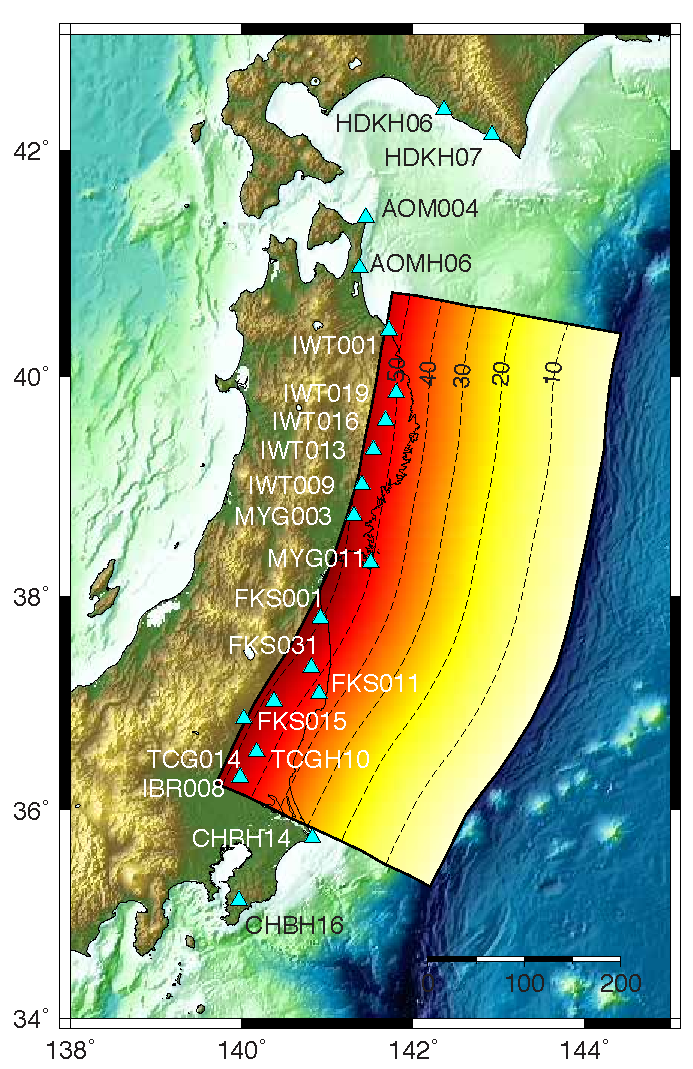
\includegraphics[width=0.55\linewidth]{./figures/ch4/kinmap.pdf}
    \caption[Station distribution for kinematic inversion]{Map of 20 stations used in the seismogeodetic slip inversion. The slab geometry used for the inversion is the same as that of Chapter 3 from \citet{hayes2012}. The contours are depth to the slab in kilometers.}
  \label{fig_kinmap}
\end{figure}

The fault model (Figure \ref{fig_kinmap}) is the same as that of Chapter 3. It is a discretized version of the Slab 1.0 model of \citep{hayes2012}. It consists of 21 along strike and 9 down-dip 25$\times$25km sub-faults (189 in total). We use a 1D layered model calibrated for Japan. The model, shown in Table \ref{tb_toku_model}, is used for automated computation of CMT's with long period data \citep{fukuyama1998,tsuruoka2009}. For the Green functions calculation we use the fk code provided by \citep{zhu2002} and compute GFs for every subfault/station pair from 0 to 0.5Hz. The data are lowpass filtered to 0.5Hz to match the GFs. We use triangular source-time functions with a 10s rise time. The maximum rupture velocity allowed is 4km/s which corresponds to 0.9 times the shear wave speed ($0.9\beta$) of the fastest layer spanned by the slab model (layer 4). We then allow slip on 20 subsequent 50\% overlapping triangle source time functions with equal rise time (10s) yielding a total of 7560 model parameters. Recall that this does not mean that rupture speed is forced to 0.9$\beta$, rather that this is the fastest possible velocity in the model. Subsequently the inversion is run using a NNLS solver to enforce positivity. To sample a large portion of the parameter space spanned by $\lambda_s$ and $\lambda_t$ we first invert on a coarse gird of smoothing parameters (between $10^{-5}$ and $10^2$). A total of 64 different $(\lambda_s,\lambda_t)$ pairs are used. We then refine the smoothing parameter grid twice more around the minimum ABIC inversion result to define the smoothing parameters that are used for final inversion.

\subsection{Kinematic Inversion Results}



\begin{table}
\caption{Velocity model for the Tohoku-oki kinematic inversion}
\label{tb_toku_model}
\begin{tabular}{l r r r r r r}
\hline
Layer & $v_p$ & $v_s$ &Density&Thickness&$Q_p$&$Q_s$\\
 & (km/s) &( km/s) & (kg/m$^{3}$) & (km) &  &\\
\hline
1 & 5.50 & 3.14 & 2.30 & 3.0 & 600 & 300\\
2 & 6.00 & 3.55 & 2.40 & 15.0 & 600 & 300\\
3 & 6.70 & 3.83 & 2.80 & 15.0 & 600 & 300\\
4 & 7.80 & 4.46 & 3.20 & 67.0 & 600 & 300\\
Half-space & 8.00 & 4.57 & 3.30 & $\infty$ & 600 & 300\\
\hline
\end{tabular}
\end{table}
%\chapter{Final notes}
%  Remove me in case of abdominal pain.

